The router is the key component of a Network-on-Chip, since it determines how flits are buffered, arbitrated, and forwarded between input and output ports. In a typical NoC router, each arriving flit first enters an input buffer, where it waits until the required output resource becomes available. Compared with traditional large-scale network routers, NoC routers are designed under much stricter latency, area, and power constraints. Therefore, their microarchitecture must provide efficient packet forwarding while keeping implementation complexity low.

The main task of the router is to transfer each incoming flit from the selected input virtual channel to the appropriate output port. To achieve this, several functions must be completed inside the router. First, the router determines the desired output direction according to the routing algorithm. For head flits, this step also identifies the candidate output virtual channels. Next, a virtual-channel allocation stage assigns an available output virtual channel to the packet. After that, switch allocation is performed to resolve contention among multiple input flits requesting the same output port. Once the allocation is granted, the flit traverses the internal crossbar and is forwarded to the output side of the router.

Figure~\ref{fig:router} shows the virtual-channel-based router architecture.

\begin{figure}[htbp]
    \centering
    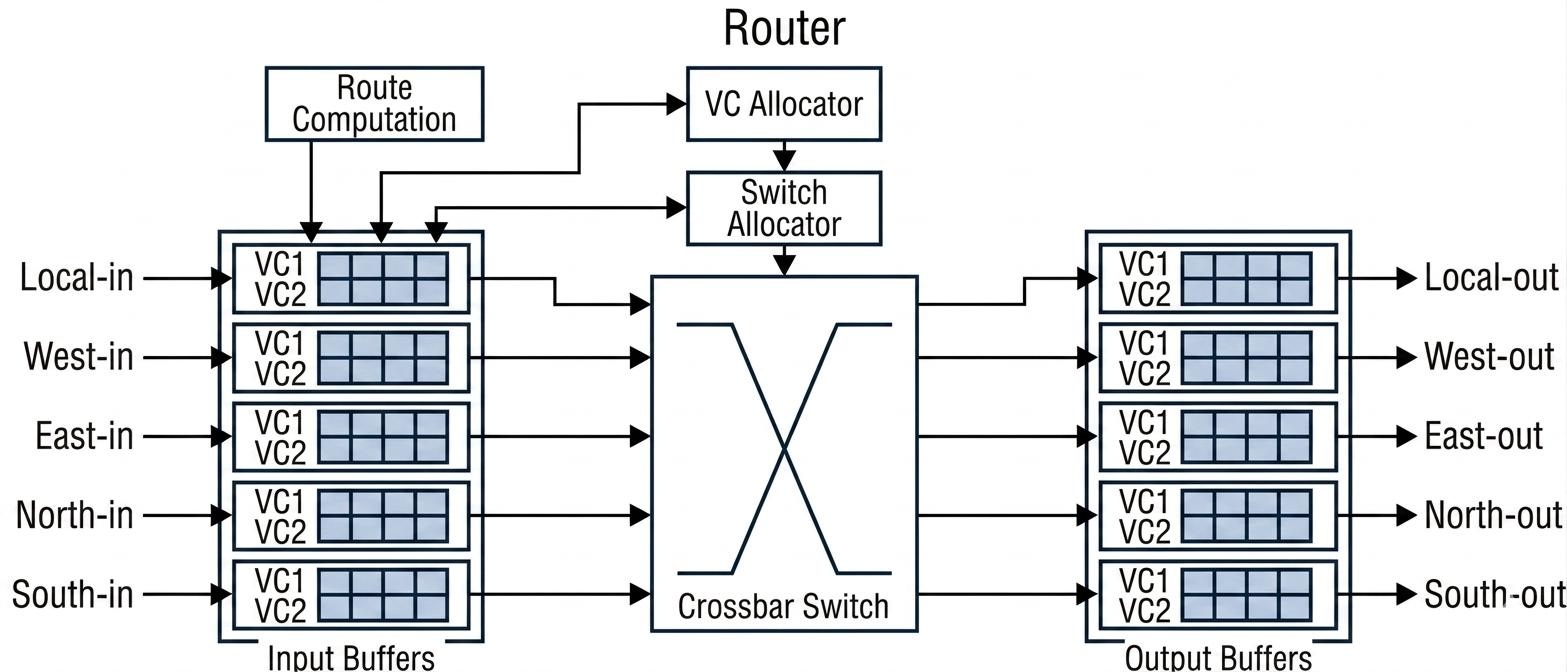
\includegraphics[width=0.85\textwidth]{images/ch2background/router.png}
    \caption{Virtual-channel-based router architecture}
    \label{fig:router}
\end{figure}

\begin{itemize}
    \item \textbf{Input buffers:}

    Input buffers temporarily store incoming flits before they are forwarded. They provide waiting space when the requested output resource is not immediately available.

    \item \textbf{Routing computation:}

    The routing computation logic determines the output port for an incoming packet according to the selected routing algorithm.

    \item \textbf{Virtual-channel allocator:}

    The virtual-channel allocator assigns an available output virtual channel to a packet, usually based on the routing result and channel availability.

    \item \textbf{Switch allocator:}

    The switch allocator resolves contention among multiple input flits requesting the same output port and decides which flit can access the crossbar in the current cycle.

    \item \textbf{Crossbar switch:}

    The crossbar switch provides the internal data path between input ports and output ports, allowing the selected flit to be transferred to its destination output.
\end{itemize}

To improve operating frequency, router operation is usually organized as a pipeline. A common pipelined flow includes buffer write, route computation, virtual-channel allocation, switch allocation and switch traversal. For body and tail flits, route computation and virtual-channel allocation are usually not repeated, since they inherit the routing and channel information established by the head flit. This reduces control overhead and improves forwarding efficiency.

Overall, router microarchitecture has a direct impact on network latency, throughput, area, and power consumption. Efficient design of buffers, allocators, and crossbar organization is therefore essential for building a practical NoC communication system.